\section{Experimental Results and Discussion}
\label{sec:results}

All four models were trained and evaluated on the class-balanced dataset (89,832 samples; $\approx$14,972 per class) using an 80/20 stratified train-test split with a 20\% validation holdout. The test set comprised 17,967 samples.

\subsection{Overall Performance Comparison}

Table~\ref{tab:results} summarises the test-set performance. BiLSTM outperformed all models ($+1.39$\,pp over CNN, $+2.13$\,pp over SVM, $+3.14$\,pp over XGBoost in accuracy). The ranking BiLSTM $>$ CNN $>$ SVM $>$ XGBoost confirmed that sequential context modelling provided a measurable advantage over local feature extraction and bag-of-words approaches.

\begin{table}[!htb]
\centering
\caption{Test-set performance comparison. All metrics are macro-averaged.}
\label{tab:results}
\small
\begin{tabular}{@{}lcccc@{}}
\toprule
\textbf{Model} & \textbf{Acc.\,(\%)} & \textbf{Prec.\,(\%)} & \textbf{Rec.\,(\%)} & \textbf{F1\,(\%)} \\
\midrule
BiLSTM   & \textbf{93.93} & \textbf{94.08} & \textbf{93.93} & \textbf{93.91} \\
CNN      & 92.54 & 92.67 & 92.54 & 92.48 \\
SVM      & 91.80 & 92.00 & 91.80 & 91.75 \\
XGBoost  & 90.79 & 90.98 & 90.79 & 90.73 \\
\bottomrule
\end{tabular}
\end{table}

\subsection{Hyperparameter Tuning}

Table~\ref{tab:hyperparams} summarises the tuning strategy and best configuration for each model. ML models used grid search with 3-fold cross-validation; DL models used EarlyStopping (patience\,=\,3, restoring best weights).

\begin{table}[!htb]
\centering
\caption{Best hyperparameter configurations per model.}
\label{tab:hyperparams}
\resizebox{\columnwidth}{!}{%
\begin{tabular}{@{}lll@{}}
\toprule
\textbf{Model} & \textbf{Search Space} & \textbf{Best Config} \\
\midrule
SVM & $C \!\in\! \{0.1, 1\}$, kernel $\!\in\!$ \{lin, rbf, poly\} & $C\!=\!1$, linear~\citep{dzikovska2012using} \\
XGBoost & lr $\!\in\! \{0.01, 0.1\}$, depth $\!\in\! \{5, 10\}$, est $\!\in\! \{50, 100\}$ & lr$\!=\!0.1$, depth$\!=\!10$, est$\!=\!100$ \\
BiLSTM & emb$\!=\!100$, 2$\times$BiLSTM (256$\!\rightarrow\!$128), drop$\!=\!0.5$ & Best ep.~3/6~\citep{sun2023bidirectional} \\
CNN & 2$\times$Conv (256$\!\rightarrow\!$128, $k\!=\!5$), drop$\!=\!0.5$ & Best ep.~3/6 \\
\bottomrule
\end{tabular}}
\end{table}

\subsection{Confusion Matrix Analysis}

Figures~\ref{fig:cm_bilstm}--\ref{fig:cm_xgboost} present confusion matrices for all four models. Two dominant misclassification patterns emerged:

\begin{enumerate}[nosep]
    \item \textbf{Joy $\leftrightarrow$ Love confusion.} All models misclassified Joy as Love (BiLSTM: 236, CNN: 255, SVM: 258, XGBoost: 246), reflecting shared positively-valenced vocabulary.
    \item \textbf{Fear $\rightarrow$ Surprise confusion.} Fear was frequently predicted as Surprise (BiLSTM: 269, CNN: 278, SVM: 275, XGBoost: 303), due to shared high-arousal lexicon (``shocked'', ``suddenly'').
\end{enumerate}

XGBoost also exhibited majority-class bias: Sadness$\rightarrow$Joy (852), Anger$\rightarrow$Joy (650), and Fear$\rightarrow$Joy (531) misclassifications.

\begin{figure*}[!htbp]
\centering
\begin{minipage}{0.48\textwidth}
  \centering
  
\includegraphics[width=\linewidth]{figures/bilstm_confusion_matrix.png}
  \captionof{figure}{BiLSTM confusion matrix.}
  \label{fig:cm_bilstm}
\end{minipage}\hfill
\begin{minipage}{0.48\textwidth}
  \centering
  
\includegraphics[width=\linewidth]{figures/cnn_confusion_matrix.png}
  \captionof{figure}{CNN confusion matrix.}
  \label{fig:cm_cnn}
\end{minipage}\\[6pt]
\begin{minipage}{0.48\textwidth}
  \centering
  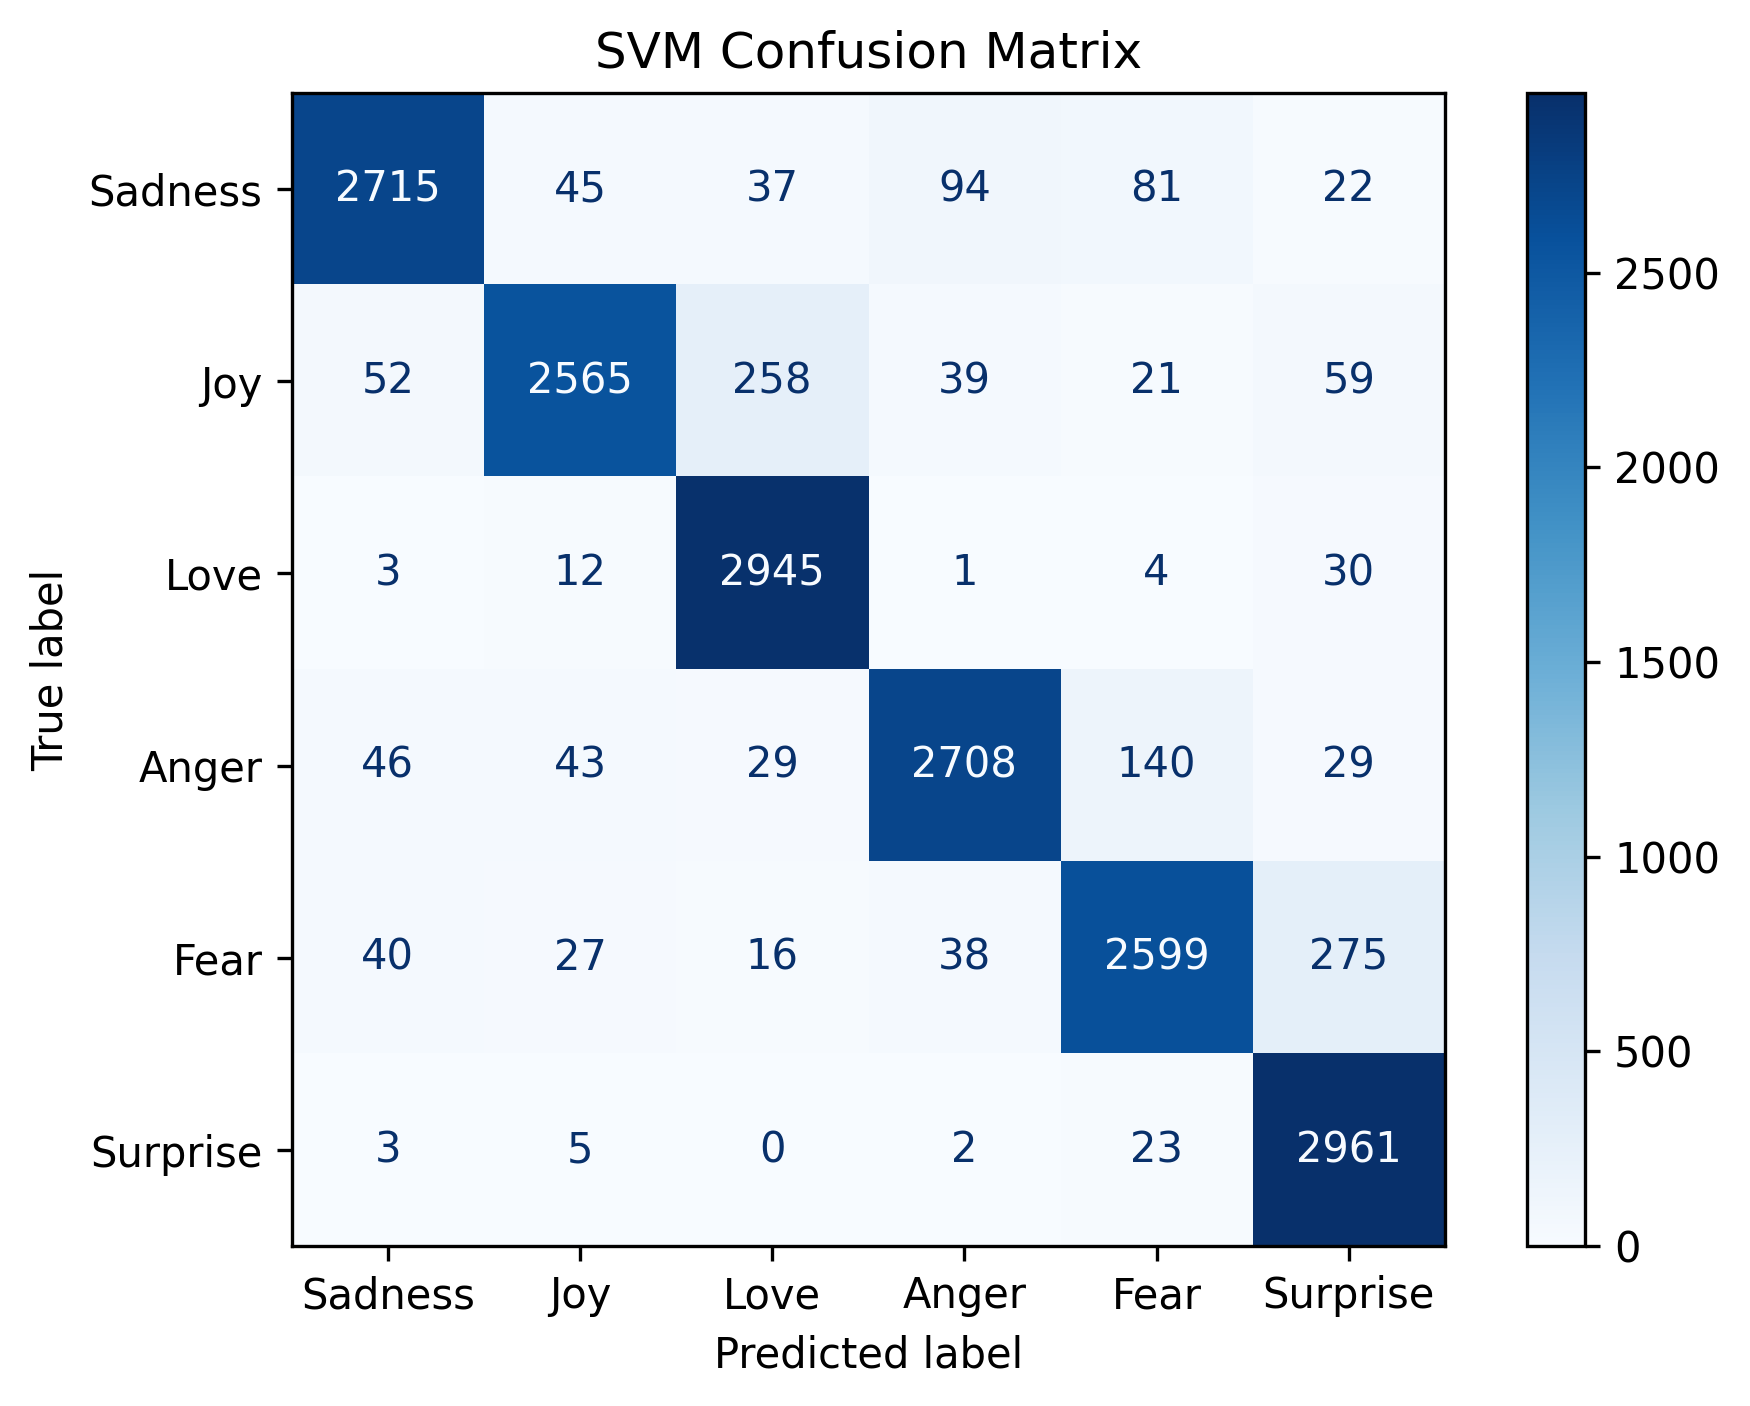
\includegraphics[width=\linewidth]{figures/svm_confusion_matrix.png}
  \captionof{figure}{SVM confusion matrix.}
  \label{fig:cm_svm}
\end{minipage}\hfill
\begin{minipage}{0.48\textwidth}
  \centering
  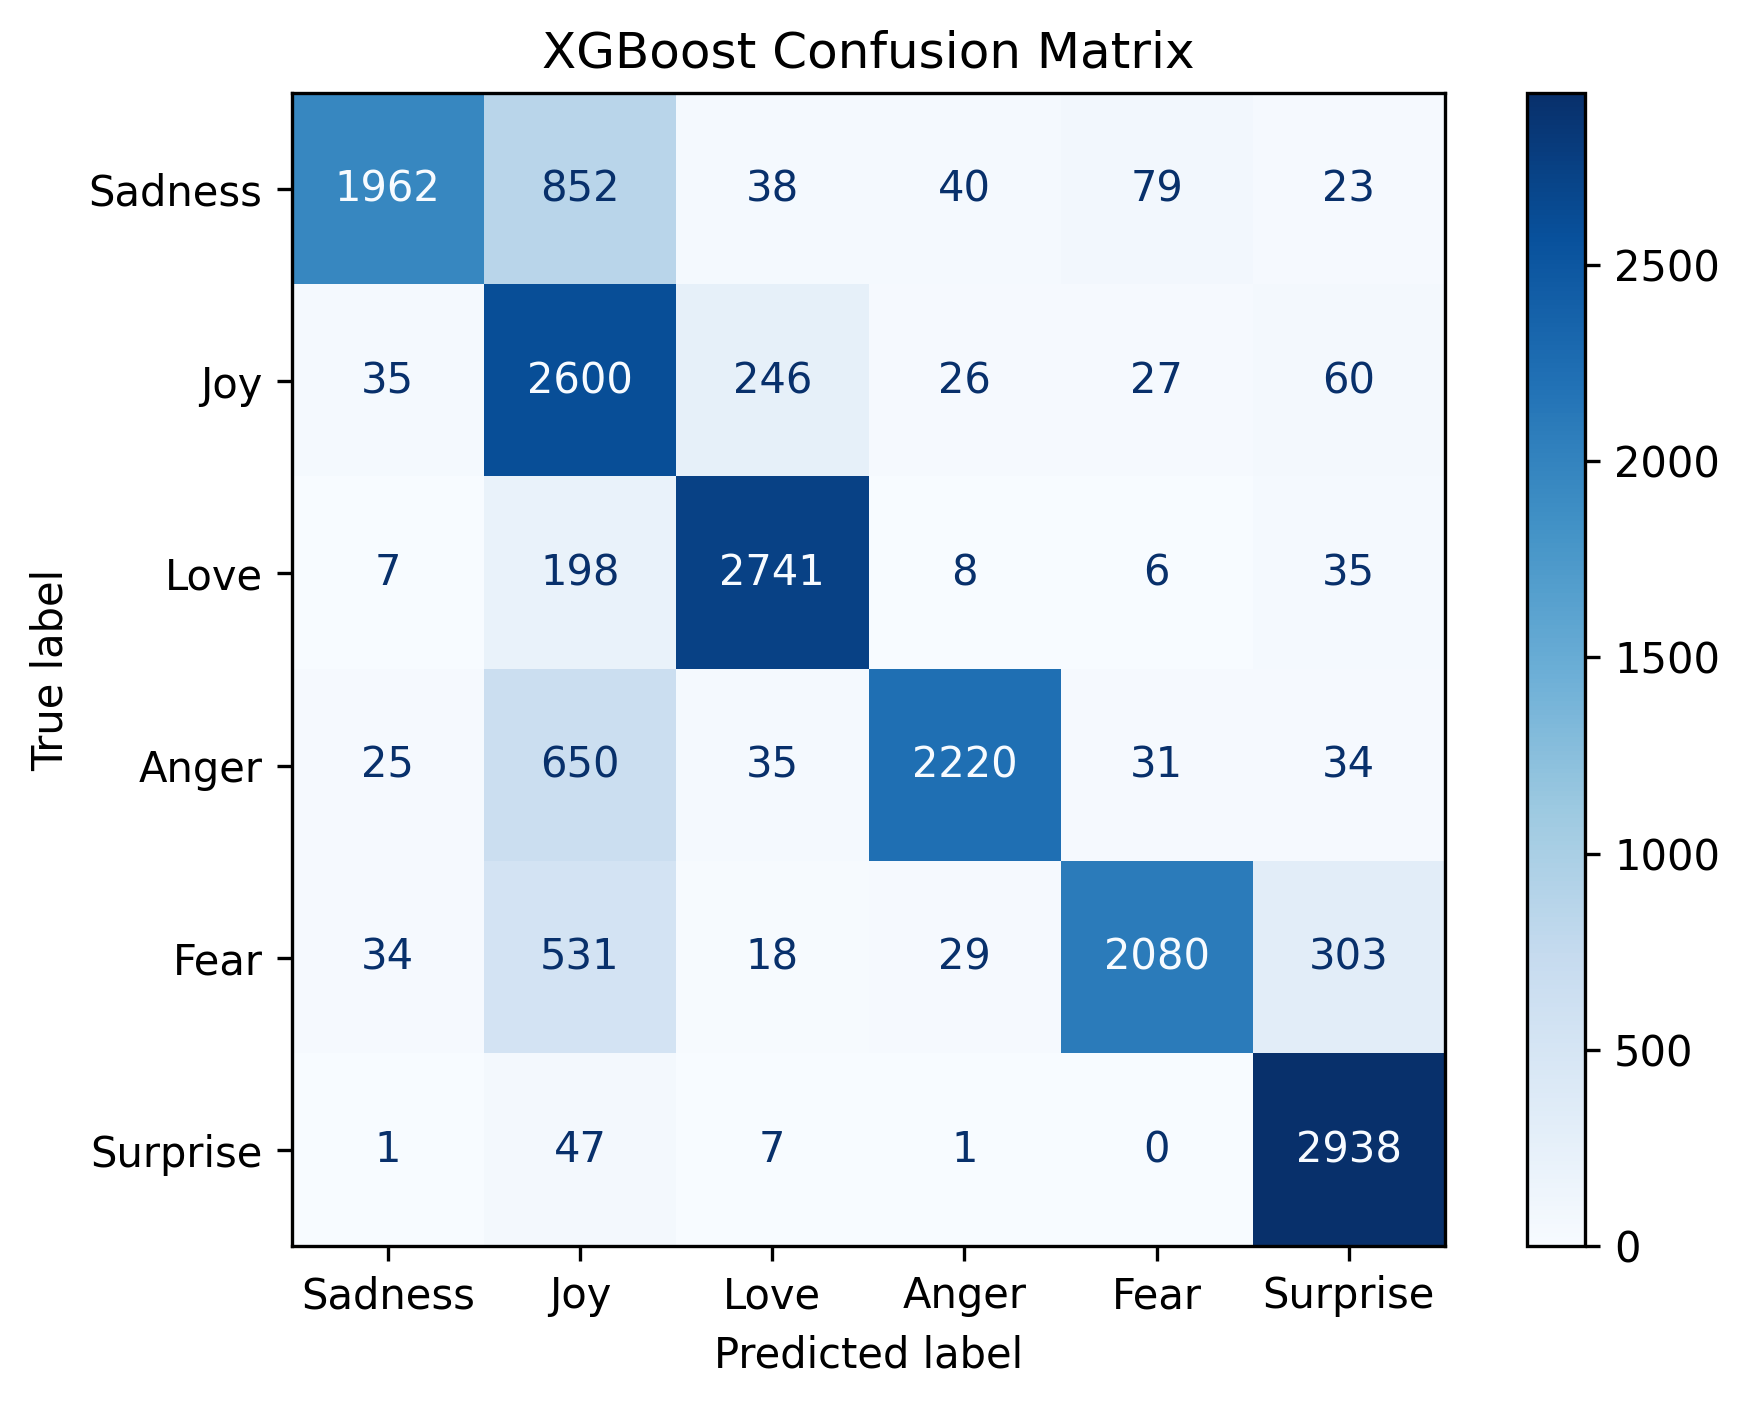
\includegraphics[width=\linewidth]{figures/xgboost_confusion_matrix.png}
  \captionof{figure}{XGBoost confusion matrix.}
  \label{fig:cm_xgboost}
\end{minipage}
\end{figure*}

\subsection{Training Dynamics and Computational Cost}

Figure~\ref{fig:train_bilstm} shows BiLSTM training curves: the model converged by epoch~3 (94.17\% validation accuracy) with a small train-val gap (${\approx}0.5$\,pp), confirming good generalisation. Figure~\ref{fig:train_cnn} shows CNN reaching 92.77\% validation accuracy at epoch~3 with early signs of overfitting.

\begin{figure*}[!htbp]
\centering
\begin{minipage}{0.48\textwidth}
  \centering
  
\includegraphics[width=\linewidth]{figures/bilstm_training_curves.png}
  \captionof{figure}{BiLSTM accuracy and loss over 6 epochs.}
  \label{fig:train_bilstm}
\end{minipage}\hfill
\begin{minipage}{0.48\textwidth}
  \centering
  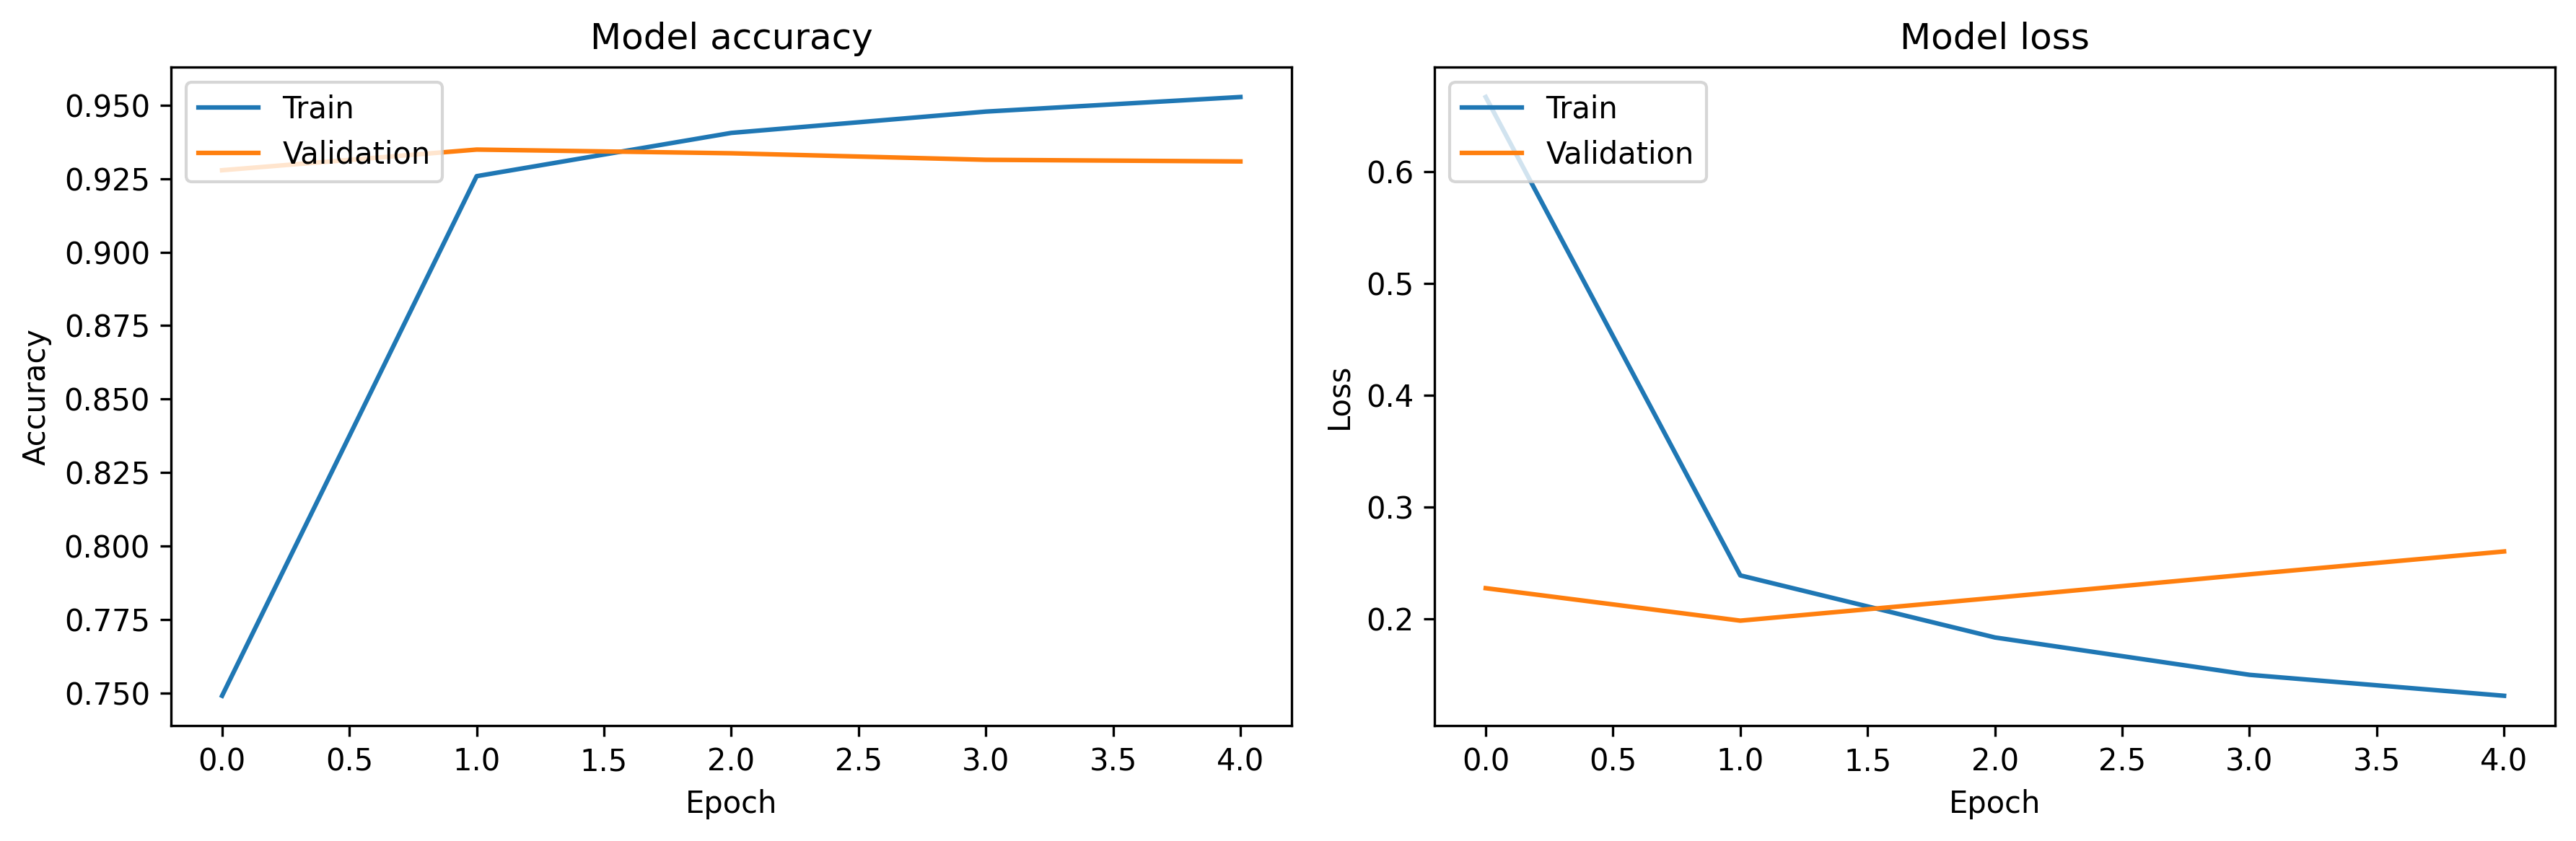
\includegraphics[width=\linewidth]{figures/cnn_training_curves.png}
  \captionof{figure}{CNN accuracy and loss over 6 epochs.}
  \label{fig:train_cnn}
\end{minipage}
\end{figure*}

Table~\ref{tab:compute} reports computational cost. SVM required the least training time while delivering the second-highest accuracy, making it the most efficient on a performance-per-compute basis. BiLSTM demanded $12\times$ the training time of SVM for a 2.13\,pp accuracy gain and ${\sim}23\times$ higher inference latency, motivating SVM's selection for deployment.

\begin{table}[!htb]
\centering
\caption{Computational cost comparison across models.}
\label{tab:compute}
\small
\begin{tabular}{@{}lccc@{}}
\toprule
\textbf{Model} & \textbf{Train Time} & \textbf{Inference} & \textbf{Model Size} \\
\midrule
SVM      & $\sim$2\,min  & $<$1\,ms/sample  & 48\,MB \\
XGBoost  & $\sim$8\,min  & $<$1\,ms/sample  & 12\,MB \\
CNN      & $\sim$2\,min (6 ep.) & $\sim$3\,ms/sample & 4.2\,MB \\
BiLSTM   & $\sim$24\,min (6 ep.) & $\sim$23\,ms/sample & 5.6\,MB \\
\bottomrule
\end{tabular}
\end{table}

\subsection{Error Analysis and Biases}

Three systematic error patterns persisted across all architectures: (1)~\textbf{valence conflation} --- Joy$\leftrightarrow$Love confusion from shared positive vocabulary (``happy'', ``amazing''); (2)~\textbf{arousal ambiguity} --- Fear$\rightarrow$Surprise errors from shared high-arousal tokens, where the two emotions differ primarily in valence; and (3)~\textbf{residual majority-class bias} in XGBoost, which still tended to misclassify negatively-valenced samples as Joy despite class-balanced training.

At the dataset level, four biases should be acknowledged: \textbf{platform bias} (Twitter-only corpus may not generalise to longer-form text); \textbf{annotation bias} from crowd-sourced labels~\citep{demszky2020goemotions}; \textbf{temporal bias} from evolving language patterns; and a \textbf{label granularity constraint} (single-label taxonomy cannot capture mixed emotions).

\subsection{Interpretability and Deployment Feasibility}

SVM offered high interpretability through its linear weight vector $w$, enabling direct feature importance analysis --- essential for clinical applications. XGBoost provided moderate interpretability via feature importance scores, while CNN and BiLSTM remained black-box classifiers. Table~\ref{tab:feasibility} summarises the deployment assessment: SVM achieved the best balance of latency, interpretability, and accuracy.

\begin{table}[!htb]
\centering
\caption{Deployment feasibility assessment across models.}
\label{tab:feasibility}
\small
\setlength{\tabcolsep}{3pt}
\begin{tabular}{@{}lcccc@{}}
\toprule
\textbf{Criterion} & \textbf{SVM} & \textbf{XGB} & \textbf{CNN} & \textbf{BiLSTM} \\
\midrule
Inference latency  & \cmark & \cmark & $\sim$ & \xmark \\
Memory footprint   & $\sim$ & \cmark & \cmark & \cmark \\
Interpretability   & \cmark & $\sim$ & \xmark & \xmark \\
Accuracy           & $\sim$ & $\sim$ & $\sim$ & \cmark \\
\bottomrule
\end{tabular}
\end{table}

SVM was deployed as a Flask REST API containerised with Docker (\texttt{python:3.11-slim}) and served via Gunicorn. The web interface provided emotion prediction with probability scores, a preprocessing trace panel, and a model performance dashboard. The Docker image (\texttt{yolandalim/125970-mindtrace:v2}) is publicly available.

\subsection{Word Cloud Visualisation}

Figure~\ref{fig:wordclouds} presents per-class word clouds. Each emotion carried distinctive vocabulary, while Fear and Surprise shared tokens such as ``suddenly'' and ``shocked'', corroborating the confusion matrix findings.

\begin{figure*}[!htbp]
\centering
\begin{minipage}{0.32\textwidth}
  \centering
  
\includegraphics[width=\linewidth]{figures/wordcloud_anger.png}\\[-2pt]
  {\small (a) Anger}
\end{minipage}\hfill
\begin{minipage}{0.32\textwidth}
  \centering
  
\includegraphics[width=\linewidth]{figures/wordcloud_fear.png}\\[-2pt]
  {\small (b) Fear}
\end{minipage}\hfill
\begin{minipage}{0.32\textwidth}
  \centering
  
\includegraphics[width=\linewidth]{figures/wordcloud_joy.png}\\[-2pt]
  {\small (c) Joy}
\end{minipage}\\[6pt]
\begin{minipage}{0.32\textwidth}
  \centering
  
\includegraphics[width=\linewidth]{figures/wordcloud_love.png}\\[-2pt]
  {\small (d) Love}
\end{minipage}\hfill
\begin{minipage}{0.32\textwidth}
  \centering
  
\includegraphics[width=\linewidth]{figures/wordcloud_sadness.png}\\[-2pt]
  {\small (e) Sadness}
\end{minipage}\hfill
\begin{minipage}{0.32\textwidth}
  \centering
  
\includegraphics[width=\linewidth]{figures/wordcloud_surprise.png}\\[-2pt]
  {\small (f) Surprise}
\end{minipage}
\caption{Per-class word clouds from the preprocessed corpus. Distinctive vocabulary per emotion; Fear and Surprise share high-arousal tokens.}
\label{fig:wordclouds}
\end{figure*}
